\documentclass{article}
\PassOptionsToPackage{numbers, sort&compress}{natbib}
\usepackage[preprint]{neurips_2020}

\usepackage[utf8]{inputenc} % allow utf-8 input
\usepackage[T1]{fontenc}    % use 8-bit T1 fonts
\usepackage{hyperref}       % hyperlinks
\usepackage{url}            % simple URL typesetting
\usepackage{booktabs}       % professional-quality tables
\usepackage{amsfonts}       % blackboard math symbols
\usepackage{nicefrac}       % compact symbols for 1/2, etc.
\usepackage{microtype}      % microtypography
\usepackage{amsmath}
\usepackage{minted}
\usepackage[table]{xcolor}% or package color
\usepackage{graphicx}
\usepackage{amssymb}
\usepackage{cancel}
\usepackage{natbib}
\usepackage{pifont}
\usepackage{bbm}
\newcommand{\cmark}{\ding{51}}%
\newcommand{\xmark}{\ding{55}}%
\usepackage{amsthm}
\usepackage{subcaption}
\usepackage{wrapfig}
\usepackage{algorithm}
\usepackage{multirow}
\usepackage{float}
\usepackage{mathtools}
\usepackage{todonotes}
\usepackage{hyperref}


\usepackage{fancyhdr}
\pagestyle{fancy}
\chead{\textsc{COS435 / ECE433: Introduction to RL}\vspace{1.2em}}
\lhead{\lectureTitle}
\rhead{\lectureDate}
% \cfoot{center of the footer!}
\renewcommand{\headrulewidth}{0.4pt}
\renewcommand{\footrulewidth}{0.4pt}

\newtheorem{theorem}{Theorem}[section]
\newtheorem{corollary}{Corollary}[theorem]
\newtheorem{lemma}[theorem]{Lemma}

% Palatino for main text and math
\usepackage[osf,sc]{mathpazo}
% Helvetica for sans serif
% (scaled to match size of Palatino)
\usepackage[scaled=0.90]{helvet}
% Bera Mono for monospaced
% (scaled to match size of Palatino)
\usepackage[scaled=0.85]{beramono}


\usepackage{amsmath,amsfonts,bm}

\newcommand{\figleft}{{\em (Left)}}
\newcommand{\figcenter}{{\em (Center)}}
\newcommand{\figright}{{\em (Right)}}
\newcommand{\figtop}{{\em (Top)}}
\newcommand{\figbottom}{{\em (Bottom)}}
\newcommand{\captiona}{{\em (a)}}
\newcommand{\captionb}{{\em (b)}}
\newcommand{\captionc}{{\em (c)}}
\newcommand{\captiond}{{\em (d)}}

\newcommand{\newterm}[1]{{\bf #1}}


\def\figref#1{figure~\ref{#1}}
\def\Figref#1{Figure~\ref{#1}}
\def\twofigref#1#2{figures \ref{#1} and \ref{#2}}
\def\quadfigref#1#2#3#4{figures \ref{#1}, \ref{#2}, \ref{#3} and \ref{#4}}
\def\secref#1{section~\ref{#1}}
\def\Secref#1{Section~\ref{#1}}
\def\twosecrefs#1#2{sections \ref{#1} and \ref{#2}}
\def\secrefs#1#2#3{sections \ref{#1}, \ref{#2} and \ref{#3}}
\def\eqref#1{equation~\ref{#1}}
\def\Eqref#1{Equation~\ref{#1}}
\def\plaineqref#1{\ref{#1}}
\def\chapref#1{chapter~\ref{#1}}
\def\Chapref#1{Chapter~\ref{#1}}
\def\rangechapref#1#2{chapters\ref{#1}--\ref{#2}}
\def\algref#1{algorithm~\ref{#1}}
\def\Algref#1{Algorithm~\ref{#1}}
\def\twoalgref#1#2{algorithms \ref{#1} and \ref{#2}}
\def\Twoalgref#1#2{Algorithms \ref{#1} and \ref{#2}}
\def\partref#1{part~\ref{#1}}
\def\Partref#1{Part~\ref{#1}}
\def\twopartref#1#2{parts \ref{#1} and \ref{#2}}

\def\ceil#1{\lceil #1 \rceil}
\def\floor#1{\lfloor #1 \rfloor}
\def\1{\bm{1}}
\newcommand{\train}{\mathcal{D}}
\newcommand{\valid}{\mathcal{D_{\mathrm{valid}}}}
\newcommand{\test}{\mathcal{D_{\mathrm{test}}}}

\def\eps{{\epsilon}}


\def\reta{{\textnormal{$\eta$}}}
\def\ra{{\textnormal{a}}}
\def\rb{{\textnormal{b}}}
\def\rc{{\textnormal{c}}}
\def\rd{{\textnormal{d}}}
\def\re{{\textnormal{e}}}
\def\rf{{\textnormal{f}}}
\def\rg{{\textnormal{g}}}
\def\rh{{\textnormal{h}}}
\def\ri{{\textnormal{i}}}
\def\rj{{\textnormal{j}}}
\def\rk{{\textnormal{k}}}
\def\rl{{\textnormal{l}}}
\def\rn{{\textnormal{n}}}
\def\ro{{\textnormal{o}}}
\def\rp{{\textnormal{p}}}
\def\rq{{\textnormal{q}}}
\def\rr{{\textnormal{r}}}
\def\rs{{\textnormal{s}}}
\def\rt{{\textnormal{t}}}
\def\ru{{\textnormal{u}}}
\def\rv{{\textnormal{v}}}
\def\rw{{\textnormal{w}}}
\def\rx{{\textnormal{x}}}
\def\ry{{\textnormal{y}}}
\def\rz{{\textnormal{z}}}

\def\rvepsilon{{\mathbf{\epsilon}}}
\def\rvtheta{{\mathbf{\theta}}}
\def\rva{{\mathbf{a}}}
\def\rvb{{\mathbf{b}}}
\def\rvc{{\mathbf{c}}}
\def\rvd{{\mathbf{d}}}
\def\rve{{\mathbf{e}}}
\def\rvf{{\mathbf{f}}}
\def\rvg{{\mathbf{g}}}
\def\rvh{{\mathbf{h}}}
\def\rvu{{\mathbf{i}}}
\def\rvj{{\mathbf{j}}}
\def\rvk{{\mathbf{k}}}
\def\rvl{{\mathbf{l}}}
\def\rvm{{\mathbf{m}}}
\def\rvn{{\mathbf{n}}}
\def\rvo{{\mathbf{o}}}
\def\rvp{{\mathbf{p}}}
\def\rvq{{\mathbf{q}}}
\def\rvr{{\mathbf{r}}}
\def\rvs{{\mathbf{s}}}
\def\rvt{{\mathbf{t}}}
\def\rvu{{\mathbf{u}}}
\def\rvv{{\mathbf{v}}}
\def\rvw{{\mathbf{w}}}
\def\rvx{{\mathbf{x}}}
\def\rvy{{\mathbf{y}}}
\def\rvz{{\mathbf{z}}}

\def\erva{{\textnormal{a}}}
\def\ervb{{\textnormal{b}}}
\def\ervc{{\textnormal{c}}}
\def\ervd{{\textnormal{d}}}
\def\erve{{\textnormal{e}}}
\def\ervf{{\textnormal{f}}}
\def\ervg{{\textnormal{g}}}
\def\ervh{{\textnormal{h}}}
\def\ervi{{\textnormal{i}}}
\def\ervj{{\textnormal{j}}}
\def\ervk{{\textnormal{k}}}
\def\ervl{{\textnormal{l}}}
\def\ervm{{\textnormal{m}}}
\def\ervn{{\textnormal{n}}}
\def\ervo{{\textnormal{o}}}
\def\ervp{{\textnormal{p}}}
\def\ervq{{\textnormal{q}}}
\def\ervr{{\textnormal{r}}}
\def\ervs{{\textnormal{s}}}
\def\ervt{{\textnormal{t}}}
\def\ervu{{\textnormal{u}}}
\def\ervv{{\textnormal{v}}}
\def\ervw{{\textnormal{w}}}
\def\ervx{{\textnormal{x}}}
\def\ervy{{\textnormal{y}}}
\def\ervz{{\textnormal{z}}}

\def\rmA{{\mathbf{A}}}
\def\rmB{{\mathbf{B}}}
\def\rmC{{\mathbf{C}}}
\def\rmD{{\mathbf{D}}}
\def\rmE{{\mathbf{E}}}
\def\rmF{{\mathbf{F}}}
\def\rmG{{\mathbf{G}}}
\def\rmH{{\mathbf{H}}}
\def\rmI{{\mathbf{I}}}
\def\rmJ{{\mathbf{J}}}
\def\rmK{{\mathbf{K}}}
\def\rmL{{\mathbf{L}}}
\def\rmM{{\mathbf{M}}}
\def\rmN{{\mathbf{N}}}
\def\rmO{{\mathbf{O}}}
\def\rmP{{\mathbf{P}}}
\def\rmQ{{\mathbf{Q}}}
\def\rmR{{\mathbf{R}}}
\def\rmS{{\mathbf{S}}}
\def\rmT{{\mathbf{T}}}
\def\rmU{{\mathbf{U}}}
\def\rmV{{\mathbf{V}}}
\def\rmW{{\mathbf{W}}}
\def\rmX{{\mathbf{X}}}
\def\rmY{{\mathbf{Y}}}
\def\rmZ{{\mathbf{Z}}}

\def\ermA{{\textnormal{A}}}
\def\ermB{{\textnormal{B}}}
\def\ermC{{\textnormal{C}}}
\def\ermD{{\textnormal{D}}}
\def\ermE{{\textnormal{E}}}
\def\ermF{{\textnormal{F}}}
\def\ermG{{\textnormal{G}}}
\def\ermH{{\textnormal{H}}}
\def\ermI{{\textnormal{I}}}
\def\ermJ{{\textnormal{J}}}
\def\ermK{{\textnormal{K}}}
\def\ermL{{\textnormal{L}}}
\def\ermM{{\textnormal{M}}}
\def\ermN{{\textnormal{N}}}
\def\ermO{{\textnormal{O}}}
\def\ermP{{\textnormal{P}}}
\def\ermQ{{\textnormal{Q}}}
\def\ermR{{\textnormal{R}}}
\def\ermS{{\textnormal{S}}}
\def\ermT{{\textnormal{T}}}
\def\ermU{{\textnormal{U}}}
\def\ermV{{\textnormal{V}}}
\def\ermW{{\textnormal{W}}}
\def\ermX{{\textnormal{X}}}
\def\ermY{{\textnormal{Y}}}
\def\ermZ{{\textnormal{Z}}}

\def\vzero{{\bm{0}}}
\def\vone{{\bm{1}}}
\def\vmu{{\bm{\mu}}}
\def\vtheta{{\bm{\theta}}}
\def\va{{\bm{a}}}
\def\vb{{\bm{b}}}
\def\vc{{\bm{c}}}
\def\vd{{\bm{d}}}
\def\ve{{\bm{e}}}
\def\vf{{\bm{f}}}
\def\vg{{\bm{g}}}
\def\vh{{\bm{h}}}
\def\vi{{\bm{i}}}
\def\vj{{\bm{j}}}
\def\vk{{\bm{k}}}
\def\vl{{\bm{l}}}
\def\vm{{\bm{m}}}
\def\vn{{\bm{n}}}
\def\vo{{\bm{o}}}
\def\vp{{\bm{p}}}
\def\vq{{\bm{q}}}
\def\vr{{\bm{r}}}
\def\vs{{\bm{s}}}
\def\vt{{\bm{t}}}
\def\vu{{\bm{u}}}
\def\vv{{\bm{v}}}
\def\vw{{\bm{w}}}
\def\vx{{\bm{x}}}
\def\vy{{\bm{y}}}
\def\vz{{\bm{z}}}

\def\evalpha{{\alpha}}
\def\evbeta{{\beta}}
\def\evepsilon{{\epsilon}}
\def\evlambda{{\lambda}}
\def\evomega{{\omega}}
\def\evmu{{\mu}}
\def\evpsi{{\psi}}
\def\evsigma{{\sigma}}
\def\evtheta{{\theta}}
\def\eva{{a}}
\def\evb{{b}}
\def\evc{{c}}
\def\evd{{d}}
\def\eve{{e}}
\def\evf{{f}}
\def\evg{{g}}
\def\evh{{h}}
\def\evi{{i}}
\def\evj{{j}}
\def\evk{{k}}
\def\evl{{l}}
\def\evm{{m}}
\def\evn{{n}}
\def\evo{{o}}
\def\evp{{p}}
\def\evq{{q}}
\def\evr{{r}}
\def\evs{{s}}
\def\evt{{t}}
\def\evu{{u}}
\def\evv{{v}}
\def\evw{{w}}
\def\evx{{x}}
\def\evy{{y}}
\def\evz{{z}}

\def\mA{{\bm{A}}}
\def\mB{{\bm{B}}}
\def\mC{{\bm{C}}}
\def\mD{{\bm{D}}}
\def\mE{{\bm{E}}}
\def\mF{{\bm{F}}}
\def\mG{{\bm{G}}}
\def\mH{{\bm{H}}}
\def\mI{{\bm{I}}}
\def\mJ{{\bm{J}}}
\def\mK{{\bm{K}}}
\def\mL{{\bm{L}}}
\def\mM{{\bm{M}}}
\def\mN{{\bm{N}}}
\def\mO{{\bm{O}}}
\def\mP{{\bm{P}}}
\def\mQ{{\bm{Q}}}
\def\mR{{\bm{R}}}
\def\mS{{\bm{S}}}
\def\mT{{\bm{T}}}
\def\mU{{\bm{U}}}
\def\mV{{\bm{V}}}
\def\mW{{\bm{W}}}
\def\mX{{\bm{X}}}
\def\mY{{\bm{Y}}}
\def\mZ{{\bm{Z}}}
\def\mBeta{{\bm{\beta}}}
\def\mPhi{{\bm{\Phi}}}
\def\mLambda{{\bm{\Lambda}}}
\def\mSigma{{\bm{\Sigma}}}

\DeclareMathAlphabet{\mathsfit}{\encodingdefault}{\sfdefault}{m}{sl}
\SetMathAlphabet{\mathsfit}{bold}{\encodingdefault}{\sfdefault}{bx}{n}
\newcommand{\tens}[1]{\bm{\mathsfit{#1}}}
\def\tA{{\tens{A}}}
\def\tB{{\tens{B}}}
\def\tC{{\tens{C}}}
\def\tD{{\tens{D}}}
\def\tE{{\tens{E}}}
\def\tF{{\tens{F}}}
\def\tG{{\tens{G}}}
\def\tH{{\tens{H}}}
\def\tI{{\tens{I}}}
\def\tJ{{\tens{J}}}
\def\tK{{\tens{K}}}
\def\tL{{\tens{L}}}
\def\tM{{\tens{M}}}
\def\tN{{\tens{N}}}
\def\tO{{\tens{O}}}
\def\tP{{\tens{P}}}
\def\tQ{{\tens{Q}}}
\def\tR{{\tens{R}}}
\def\tS{{\tens{S}}}
\def\tT{{\tens{T}}}
\def\tU{{\tens{U}}}
\def\tV{{\tens{V}}}
\def\tW{{\tens{W}}}
\def\tX{{\tens{X}}}
\def\tY{{\tens{Y}}}
\def\tZ{{\tens{Z}}}


\def\gA{{\mathcal{A}}}
\def\gB{{\mathcal{B}}}
\def\gC{{\mathcal{C}}}
\def\gD{{\mathcal{D}}}
\def\gE{{\mathcal{E}}}
\def\gF{{\mathcal{F}}}
\def\gG{{\mathcal{G}}}
\def\gH{{\mathcal{H}}}
\def\gI{{\mathcal{I}}}
\def\gJ{{\mathcal{J}}}
\def\gK{{\mathcal{K}}}
\def\gL{{\mathcal{L}}}
\def\gM{{\mathcal{M}}}
\def\gN{{\mathcal{N}}}
\def\gO{{\mathcal{O}}}
\def\gP{{\mathcal{P}}}
\def\gQ{{\mathcal{Q}}}
\def\gR{{\mathcal{R}}}
\def\gS{{\mathcal{S}}}
\def\gT{{\mathcal{T}}}
\def\gU{{\mathcal{U}}}
\def\gV{{\mathcal{V}}}
\def\gW{{\mathcal{W}}}
\def\gX{{\mathcal{X}}}
\def\gY{{\mathcal{Y}}}
\def\gZ{{\mathcal{Z}}}

\def\sA{{\mathbb{A}}}
\def\sB{{\mathbb{B}}}
\def\sC{{\mathbb{C}}}
\def\sD{{\mathbb{D}}}
\def\sF{{\mathbb{F}}}
\def\sG{{\mathbb{G}}}
\def\sH{{\mathbb{H}}}
\def\sI{{\mathbb{I}}}
\def\sJ{{\mathbb{J}}}
\def\sK{{\mathbb{K}}}
\def\sL{{\mathbb{L}}}
\def\sM{{\mathbb{M}}}
\def\sN{{\mathbb{N}}}
\def\sO{{\mathbb{O}}}
\def\sP{{\mathbb{P}}}
\def\sQ{{\mathbb{Q}}}
\def\sR{{\mathbb{R}}}
\def\sS{{\mathbb{S}}}
\def\sT{{\mathbb{T}}}
\def\sU{{\mathbb{U}}}
\def\sV{{\mathbb{V}}}
\def\sW{{\mathbb{W}}}
\def\sX{{\mathbb{X}}}
\def\sY{{\mathbb{Y}}}
\def\sZ{{\mathbb{Z}}}

\def\emLambda{{\Lambda}}
\def\emA{{A}}
\def\emB{{B}}
\def\emC{{C}}
\def\emD{{D}}
\def\emE{{E}}
\def\emF{{F}}
\def\emG{{G}}
\def\emH{{H}}
\def\emI{{I}}
\def\emJ{{J}}
\def\emK{{K}}
\def\emL{{L}}
\def\emM{{M}}
\def\emN{{N}}
\def\emO{{O}}
\def\emP{{P}}
\def\emQ{{Q}}
\def\emR{{R}}
\def\emS{{S}}
\def\emT{{T}}
\def\emU{{U}}
\def\emV{{V}}
\def\emW{{W}}
\def\emX{{X}}
\def\emY{{Y}}
\def\emZ{{Z}}
\def\emSigma{{\Sigma}}

\newcommand{\etens}[1]{\mathsfit{#1}}
\def\etLambda{{\etens{\Lambda}}}
\def\etA{{\etens{A}}}
\def\etB{{\etens{B}}}
\def\etC{{\etens{C}}}
\def\etD{{\etens{D}}}
\def\etE{{\etens{E}}}
\def\etF{{\etens{F}}}
\def\etG{{\etens{G}}}
\def\etH{{\etens{H}}}
\def\etI{{\etens{I}}}
\def\etJ{{\etens{J}}}
\def\etK{{\etens{K}}}
\def\etL{{\etens{L}}}
\def\etM{{\etens{M}}}
\def\etN{{\etens{N}}}
\def\etO{{\etens{O}}}
\def\etP{{\etens{P}}}
\def\etQ{{\etens{Q}}}
\def\etR{{\etens{R}}}
\def\etS{{\etens{S}}}
\def\etT{{\etens{T}}}
\def\etU{{\etens{U}}}
\def\etV{{\etens{V}}}
\def\etW{{\etens{W}}}
\def\etX{{\etens{X}}}
\def\etY{{\etens{Y}}}
\def\etZ{{\etens{Z}}}

\newcommand{\pdata}{p_{\rm{data}}}
\newcommand{\ptrain}{\hat{p}_{\rm{data}}}
\newcommand{\Ptrain}{\hat{P}_{\rm{data}}}
\newcommand{\pmodel}{p_{\rm{model}}}
\newcommand{\Pmodel}{P_{\rm{model}}}
\newcommand{\ptildemodel}{\tilde{p}_{\rm{model}}}
\newcommand{\pencode}{p_{\rm{encoder}}}
\newcommand{\pdecode}{p_{\rm{decoder}}}
\newcommand{\precons}{p_{\rm{reconstruct}}}

\newcommand{\laplace}{\mathrm{Laplace}} %

\newcommand{\E}{\mathbb{E}}
\newcommand{\Ls}{\mathcal{L}}
\newcommand{\R}{\mathbb{R}}
\newcommand{\emp}{\tilde{p}}
\newcommand{\lr}{\alpha}
\newcommand{\reg}{\lambda}
\newcommand{\rect}{\mathrm{rectifier}}
\newcommand{\softmax}{\mathrm{softmax}}
\newcommand{\sigmoid}{\sigma}
\newcommand{\softplus}{\zeta}
\newcommand{\KL}{D_{\mathrm{KL}}}
\newcommand{\Var}{\mathrm{Var}}
\newcommand{\standarderror}{\mathrm{SE}}
\newcommand{\Cov}{\mathrm{Cov}}
\newcommand{\normlzero}{L^0}
\newcommand{\normlone}{L^1}
\newcommand{\normltwo}{L^2}
\newcommand{\normlp}{L^p}
\newcommand{\normmax}{L^\infty}

\newcommand{\parents}{Pa} %

\DeclareMathOperator*{\argmax}{arg\,max}
\DeclareMathOperator*{\argmin}{arg\,min}

\DeclareMathOperator{\sign}{sign}
\DeclareMathOperator{\Tr}{Tr}
\let\ab\allowbreak



\title{\lectureTitle}

\begin{document}


\newcommand{\lectureTitle}{Optimal Option Pricing and Hedging}
\newcommand{\lectureDate}{Due: May 11th, 10:30 PM}

\textsc{COS435 / ECE433: Introduction to RL} 
\vspace{1em} \hfill \lectureDate

\maketitle

\paragraph{Authors.} Arif Ansari (\textit{aa4433@princeton.edu}), Jeremy Bird (\textit{jb9895@princeton.edu}), Christos Avgerinos Tegopoulos (\textit{ct3125@princeton.edu})

\paragraph{Link to GitHub Repo.} [need to change repo to public, my key is broken]

\section{Introduction}

\textbf{Motivation:} Financial markets have undergone a large degree of electronification in recent decades. The availability of high-quality data has enabled new participants to enter, leveraging sophisticated infrastructure and models to capture the lion's share of the market. Perhaps no area has been more impacted than options market making, where High Frequency Trading giants, such as Optiver, Jane Street and Jump Trading dominate competition. As trading volumes increase, one of the biggest challenges for these companies is managing inventory risk. In an ideal world market makers would always be market-neutral, but in practice, they oftentimes have to warehouse a lot of risk on their trading books due to imbalances throughout the day.\\\\
Options traders and market makers are often termed "volatility traders", since they trade these instruments as a means of getting exposure to the volatility of the underlying asset. To that end, they do not want to have exposure to movement of the underlying itself, since it is less predictable than the volatility and introduces a lot of risk onto their books. In order to achieve that, they need to take an offsetting position in the underlying asset, such that their portfolio is momentarily risk-less, and adjust their position according to the evolution of the underlying asset.\\\\
\textbf{The Problem:}
Consider the following setup. You are a trader at a large Wall Street bank that has sold 100 call options to one of its hedge fund clients. Call options are a form of derivative securities which give the holder the right but not the obligation to purchase a certain asset at a predetermined strike price K at expiration. Their payoffs are:
\begin{equation}
    C = (S_T-K)^+
\end{equation}
where $S_T$ is the terminal price of the underlying and $K$ is the strike price. Since you are selling 100 of these contracts, your exposure as a trader is $-100C$. Being risk averse, you want to hedge your position. On the other hand, you are a trader; literally in the business of making money, so you want to do so by paying as little as you can. This is not a trivial problem. A naive approach would be to just hold $100\Delta$ units of the underlying, such that $\Delta = \partial C/\partial S$. There are a few problems with this. Firstly, how should one calculate the partial derivative of the call price with respect to its underlying? This would require an analytical expression of the call price as a function of the underlying price. Moreover, whatever analytical solution we arrive at will be model dependent, and a function of the volatility of the underlying asset. Simplified models assume constant volatility, and hence geometric brownian motion, however there is strong empirical evidence to suggest that stock returns have heavy tails, and thus are driven by a stochastic volatility process. Additionally, this approach would only work if the trader is somehow able to continuously adjust their position. In practice, they might only be able to do so in sparse intervals, potentially at the end of each trading day. Finally, when a trader actually proceeds to execute their hedge at the market, they have to pay transaction costs. These transaction costs are made up from the bid-ask spread, the different between the price paid to sell / buy a stock, as well as liquidity costs, particularly important for less frequently traded options contracts.\\\\
A robust model should take all the above considerations into account. The point around transactions costs in particular moves this away from an optimal control or a bandit problem, and makes it a suitable candidate for a reinforcement learning approach. In developing the methodology for this paper, we first explore how the solution to this problem has evolved over the years, starting from the Black-Scholes-Merton model all the way to modern Reinforcement Learning research being undertaken in the field.\\\\
\textbf{Previous Proposed Solutions:}\\\\
\textit{Black Scholes}\\Fischer Black and Myron Scholes were the first to provide a solution to this problem. Their revolutionary paper \cite{bsm} came out in the 1973 and allowed the options market to grow to the multi-trillion dollar market it is today. They proved that under a certain set of assumptions; frictionless continuous trading, no arbitrage, as well as log-normal asset prices, that call prices are given by:
\begin{equation}
    C = SN(d_1)-Ke^{-r(T-t)}N(d_2)
\end{equation}
where $d_{1,2}$ are given by:
\begin{equation}
    d_{1,2} = \frac{log(\frac{S}{K})+(r\pm\frac{\sigma^2}{2})(T-t)}{\sigma\sqrt{T-t}}
\end{equation}
In this model, pricing an option is synonymous to obtain the optimal hedge, because one can simply set $\Delta = \frac{\partial C}{\partial S} = N(d_1)$ and obtain an analytical solution to the problem.\\\\
\textit{Bartlett's Delta}\\One of the more glaring failures of the BS model, is its failure to take into account the stochastic nature of the volatility process governing the underlying stock dynamics. In the BS model, the stock follows a log-normal process, given by:
\begin{equation}
    dS_t = \mu S_tdt+\sigma S_tdW_t
\end{equation}
where $S_t$ is the underlying stock price, $\mu, \sigma$ are the drift rate and volatility respectively, and $W_t$ is Standard Brownian Motion.\\\\
A more realistic representation of a stock process is the SABR model \cite{bartlett}. A simplified representation, setting the hyperparameter $\beta = 1$ is as follows:
\begin{align}
dS_t = \sigma_tS_tdW_t\label{eq:spot}\\
d\sigma_t=\alpha\sigma_tdB_t\\
dW_tdB_t = \rho dt
\end{align}
Essentially, both the stock price and volatility processes are driven by two brownian motions that are correlated by a factor $\rho$ which is typically $<0$.\\\\
Under this model, the modified $\Delta$ is given by:
\begin{equation}
    \Delta^{mod}_t = \frac{\partial C}{\partial S} +\frac{\partial C}{\partial \sigma} \bigg( \eta + \text{SABR term}\bigg)
\end{equation}
This modified Delta is called \textit{Bartlett's Delta} and is often used by practitioners to account for the deviations from the BS Delta under more realistic volatility models. Despite this improvement, the model assumes continuous, frictionless trading, requiring further work.
\\\\
\textit{Q-Learner Black Scholes (QLBS)}\\Igor Halperin lays the foundations for Reinforcement Learning - based approaches in tackling this problem with his paper published in 2020\cite{halperin}. It discretizes and constructs a risk-adjusted Markov Decision Process version of the classical BS model. This risk-adjusted version places a risk-averse trader as the agent, who on one hand wants to minimize risk, measured by the variance of the hedged portfolio, but also cares about their expected returns. This can be solved as an optimal control problem under the Mean-Variance Markowitz framework, and similarly provides an analytical solution for $\Delta$:
\begin{equation}
    \Delta_{QLBS} = \frac{\partial C}{\partial S} +\frac{\mu - r}{2\lambda \sigma^2}\frac{1}{S_t}
\end{equation}
Clearly, the deviation from optimal BS hedging arises from the difference between the expected drift $\mu$ and r, as well as the risk aversion parameter $\lambda$. This provides us with some useful intuitions for our further work. Unfortunately, this problem was again solved in a model-dependent setting, without an accurate model of the underlying stock dynamics. More importantly, there was never an attempt to train an RL agent to solve this problem.
\\\\
\textit{Reinforcement Learning}\\
Following the work of Halperin, several papers built on the QLBS framework of representing the problem as a risk-adjusted MDP with training a Reinforcement Learning model to solve the problem\cite{cao}\cite{stoiljkovic}\cite{du}. Not only so, but the RL models are trained on data generated through a more realistic stochastic volatility process as well as modeling transaction costs, resulting in a more robust representation of the real world.\\\\
An important element that we directly adopt in our method is the accounting PnL formulation of the reward function used in \cite{cao}. Using the above, and a similar Markowitz Mean-Variance framework for the objective function, a RL agent was successfully trained via DDPG. 
\section{Methods}

\textbf{Data Generating Process(DGP):} The first challenge in developing our own method to implement a RL model is collecting data. Options data in particular is relatively inaccessible, and synchronizing stock and option time-series for a given ticker is an additional challenge. Also, we wanted to benchmark our model against certain parametrized models, which require knowledge of the underlying dynamics.To that end, we decided to simulate stock data. The trajectories are shown below:\\
\begin{figure}[h!]
    \centering
    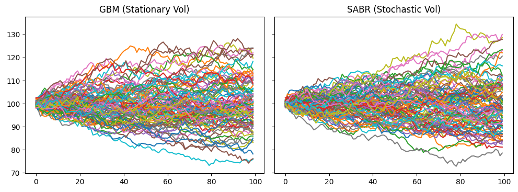
\includegraphics[width=\linewidth]{figures/trajectories.png}
    \caption{Simulated stock trajectories under different volatility assumptions}
    \label{fig:trajectory}
\end{figure}\\
Two different models were used. The first was a discretized version of the log-normal stock dynamics used in BS. Equation  \ref{eq:spot} can be discretized into:
\begin{equation}
    S_{t+1} = S_t*exp(0.5\sigma^2dt+\sigma\sqrt{dt}Z)
\end{equation}
where $Z\sim N(0,1)$. It is important to note that there are the dynamics under the risk neutral measure $\hat{P}$, and that we've set $r = \mu = 0$.\\\\
The second set of simulated stock data were generated under stochastic volatility assumptions. A discretized version of the SABR model\cite{hagan} was used, such that:\\
\begin{align}
N_1 = Z_1\\
N_2 = \rho Z_1+\sqrt{1-\rho^2}Z_2\\
S_{t+1} = S_t*exp(0.5\sigma_t^2dt+\sigma_t\sqrt{dt}N_1)\\
\sigma_{t+1} = \sigma_t*exp(0.5\nu^2dt+\nu\sqrt{dt}N_2)
\end{align}
where $Z_1\sim N(0,1), Z_2\sim N(0,1), Z_1 \perp Z_2$.\\\\
One and three month options contracts tend to be the most frequently traded and liquid. To that end, we simulate corresponding paths for the underlying for one and three month durations. In order to strike a reasonable balance between computational complexity and a realistic representation of the real world, we set our hedging frequency, and thus the time step of our simulation, to be daily. Hence, $dt \approx \frac{1}{252}$, which is one divided by the number of trading days in a year.\\

\textbf{Environment Setup:} The \textbf{gym} module was used to setup an appropriate environment for this problem. The setup is as follows:
\begin{itemize}
    \item \textbf{State:} The state is 4 dimensional array, consisting of the current stock price $S_t$, the current volatility $\sigma_t$, the current action taken $a_t$ as well as the portion of the trajectory remaining $\tau_t$. These 4 variables would be representative of an observable set of inputs available to a trader on the job.
    \item \textbf{Action:} The action is the amount of underlying stock purchased for hedging purposes. Since we are selling 100 options contracts, and we know analytically that $\Delta \in[0,1]$, we constrain our action space $a_t \in[0, 100]$.
    \item \textbf{Reward:} The accounting PnL as used in the Cao paper\cite{cao} is used as the reward at time t. \begin{equation}
        r_{t+1} = a_{t}(S_{t+1}-S_t)-(C_{t+1}-C_t)-\kappa|S_{t+1}(a_{t+1}-a_t)|
    \end{equation}
    The first term accounts for the profits realized from the hedge position, the second is simply minus the change in the call price, while the third accounts for transaction costs, which scale linearly with the amount of underlying purchased.
\end{itemize}
From there, we finally define an objective function in the Markowitz Mean-Variance framework. For each trajectory, we first evaluate the total rewards $R_t = \sum_{i = t}^{i = T} r_i$. It is important to note that we don't use any discounting $\gamma$, as we equally care about the PnL throughout the episode.\\\\
An important feature of the environment, is that the Objective in not to maximize the rewards. As mentioned earlier, we are putting on the shoes of a risk-averse trader, and hence have a tradeoff between the mean and standard deviation of the rewards of our trajectories. The objective function can be expressed as follows:
\begin{equation}
    \max_{a\sim \pi, s\sim p(s|a)}\mathbb{E}[R_0]- \lambda\sqrt{(\mathbb{E}[R_0^2]-\mathbb{E}[R_0]^2)}
\end{equation}
\textbf{Reinforcement Learning Model:} A DDPG model \cite{lillicrap} was trained to solve this model. In order to capture both the mean and variance of the cumulative rewards for each trajectory, we have elected to use two critic functions, each evaluating separate components of our Reinforcement Learning objective.\\\\
More specifically, $Q_1$ is used to evaluate the first moment of the rewards of each trajectory $R_t$, while $Q_2$ evaluates the second moment $R_t^2$. The Q-Functions for each critic are described by the following Bellman equations:
\begin{align}
    Q_1(s_t, a_t)&=r_t+\gamma *Q_1(s_{t+1}, a_{t+1})\\
    Q_2(s_t,a_t) &= (Q_1(s_t, a_t))^2\\
    &= (r_t+\gamma *Q_1(s_{t+1}, a_{t+1}))^2\\
    &= r_t^2+2r_t\gamma*Q_2(s_t,a_t)+\gamma^2 *Q_1(s_{t+1}, a_{t+1})
\end{align}
Both Q-Fuctions at time $t$ are linear functions of the reward at time $t$ and Q-Functions at the subsequent time step; $t+1$. This allows us to use the DDPG update rule to learn them over the course of training.\\\\
In parallel, in accordance with DDPG, we also updates our actor at each iteration of training to maximize the objective function stated above, or equivalently minimize the loss function:
\[
\max_{\pi} \ Q_1 - \lambda \sqrt{Q_2-Q_1^2}  \quad \Rightarrow \quad \min_{\pi} \ \mathcal{L} := - \left(Q_1 - \lambda \sqrt{Q_2-Q_1^2}\right)
\]

\textbf{Behavioral Cloning Hot-Start:} The problem we are trying to solve is very complex, and hence training a RL model will be very computationally expensive. A proposed solution to this problem was "hot-starting" our model using Behavioral Cloning.\\\\
\textit{Actor}\\
When implementing Behavioral Cloning, we need expert samples to train our model. While we don't have data from experienced traders, analytical solutions should be a good enough to get the model performing to a strong baseline. Referring to the earlier section on Previous Proposed Solutions, there are two analytical solutions available to us, based on either the BS Delta, or Bartlett's Delta. The choice of expert sample depends on the underlying dynamics of the stock data. For log-normal dynamics, we use the BS Delta, while for stochastic volatility dynamics, we use Bartlett's Delta. The expert actions are thus given as follows:
\begin{equation}
    \text{Constant Vol: } a_{expert}=100\cdot \Delta^{BS}_t, \text{Stochastic Vol: }a_{expert} = 100\cdot\Delta_t^{mod}
\end{equation}
\textit{Critic}\\
Despite "hot-starting" our actor using the method above, both critic functions $Q_1, Q_2$ have not been trained. As a result, we cannot yet proceed to train our model through DDPG, as the critic function being unstable would likely incorrectly evaluate the efficacy of our policy, causing our policy to deteriorate from the local minimum we have reached.\\\\
In order to do so, we train the model as normal, but add Gaussian noise to the action selected by our policy and temporarily halt the learning for our actor. This allows us to only update the critic during this stage, while the noise aids with the exploration of the state - action space.
\section{Results}
The model was tested in a variety of different environments. The parameters varied included the volatility dynamics, the tenor of the option, as well as wether the model was "hot-started". On top of comparing the model performance across these different parameters, the model was also benchmarked against the analytical solutions used to generate the expert dataset, as well as the policy of not hedging at all, i.e. $\pi(a|s) = 0$  $\forall s$.\\\\
\textit{Constant Volatility - Lognormal dynamics}\\
We begin by evaluating our model under the simplifying assumption of stochastic volatility. The analytical solution this is benchmarked against, which is then used to train hot-started model is thus the BS delta $\Delta^{BS}$. Clearly, as can be seen in the figure below, the model is able to learn at a slow but stable rate. It strongly outperforms the policy of not hedging, and even boasts modest outperformance of the analytical solution. The hot and cold started models converge to a similar performance, however the hot-started model is able to do so in much fewer iterations.\\
\begin{figure}[h!]
    \centering
    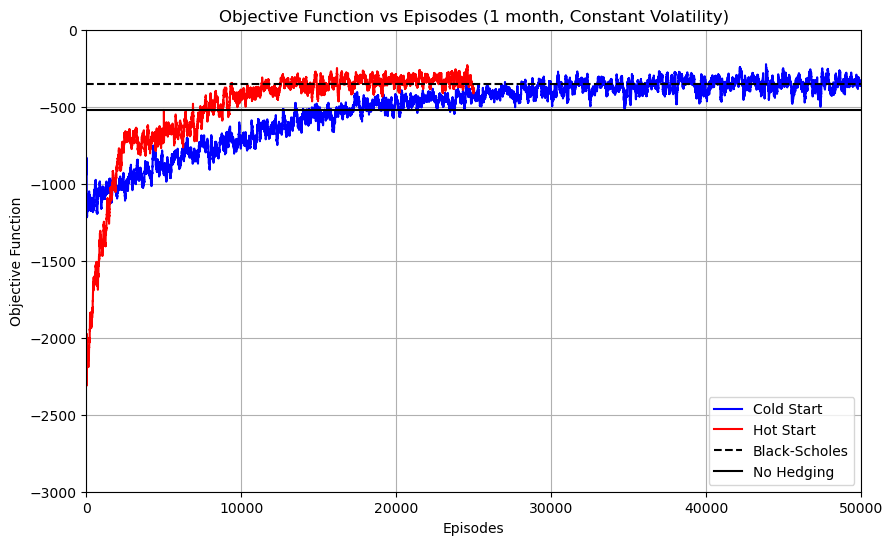
\includegraphics[width=.9\linewidth]{figures/1m_const.png}
    \caption{Training curves for 1-month options w/ constant volatility}
    \label{fig:1m_const}
\end{figure}\\
Subsequently, the performance of the same model was evaluated for the 3-month expiry options. The training curves converge to a smaller value for the objective function which is reasonable, as more transaction costs accumulate over the longer trajectories. Despite the cold-started model remaining stable over the course of training, we observe sharp drops in performance for the hot-started model. This effect can be attributed to the more pronounced temporal dislocation between the actions taken and the eventual rewards. Not only so, but since the variance of the underlying stock scales with time, the state space is enriched, requiring more samples for learning.\\
\begin{figure}[H]
    \centering
    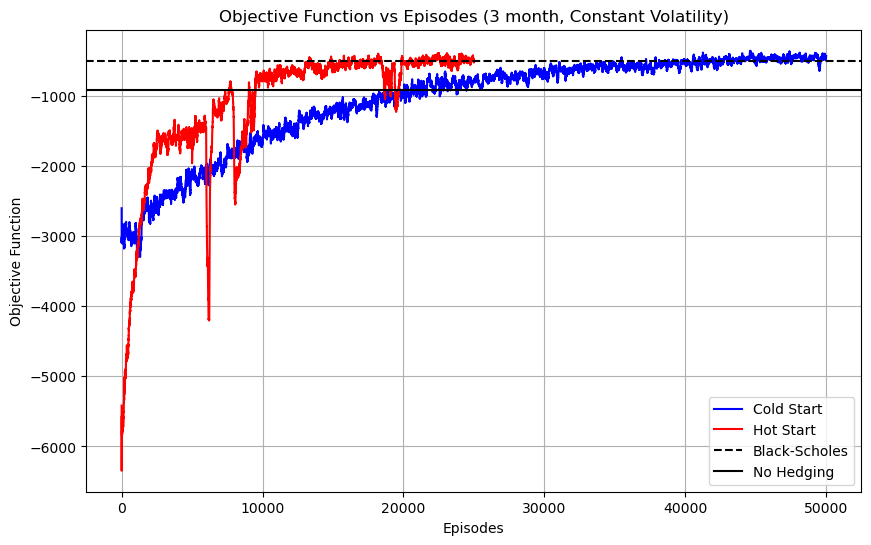
\includegraphics[width=.9\linewidth]{figures/3m_const.png}
    \caption{Training curves for 3-month options w/ constant volatility}
    \label{fig:3m_const}
\end{figure}
\textit{Stochastic Volatility - SABR dynamics}\\
The same exercise is repeated, only this time under stochastic volatility dynamics. In this more realistic environment, we opt to use the Bartlett Delta as the corresponding analytical benchmark, as well as the expert actor used to hot-start our models. The training curves are as follows:\\
\begin{figure}[h!]
    \centering
    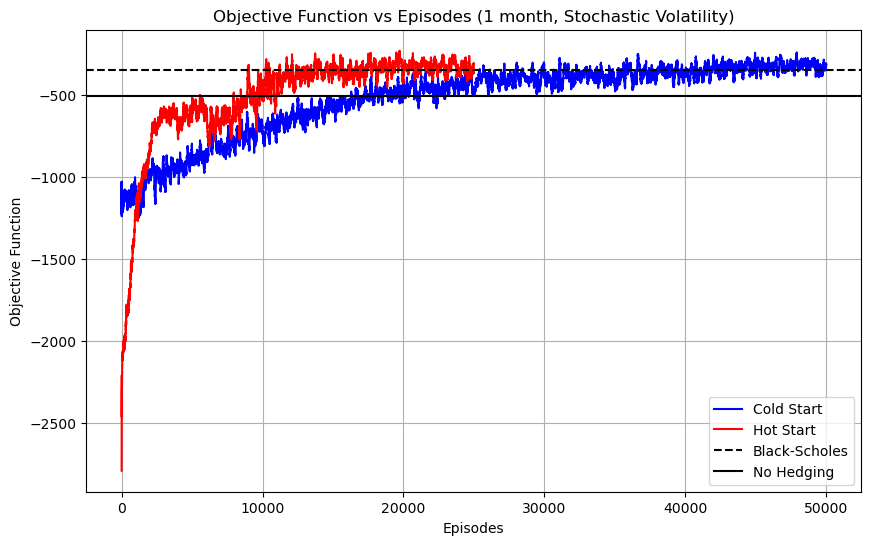
\includegraphics[width=.9\linewidth]{figures/1m_stoch.png}
    \caption{Training curves for 1-month options w/ stochastic volatility}
    \label{fig:1m_stoch}
\end{figure}\\
\begin{figure}[h!]
    \centering
    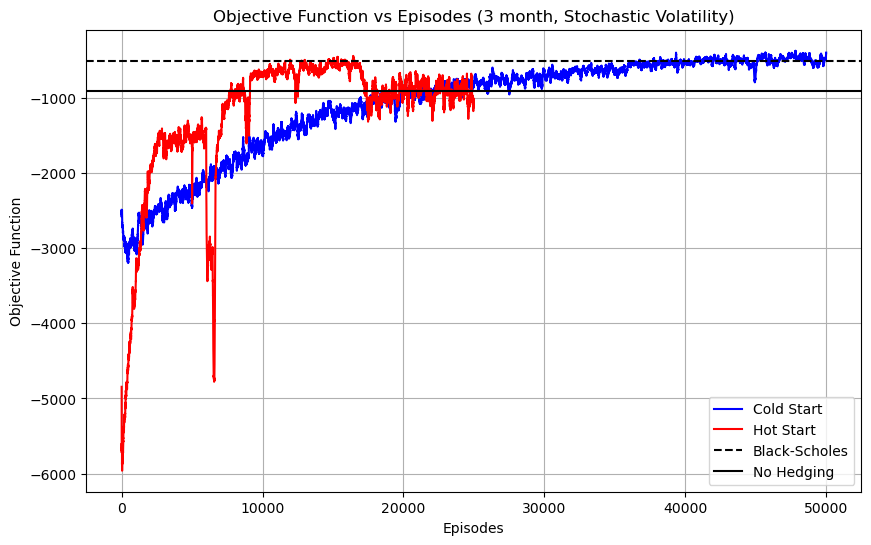
\includegraphics[width=.9\linewidth]{figures/3m_stoch.png}
    \caption{Training curves for 3-month options w/ stochastic volatility}
    \label{fig:3m_stoch}
\end{figure}\\
Overall, the observations we make are in line with the constant volatility environment. Notably, the out-performance compared to the analytical benchmarks is stronger in the 1-month stochastic compared to the 1-month lognormal case. On the other hand, the training curve appears even more unstable for the hot-started 3 month curve, and appears to get stuck at a local minima after seemingly converging in performance close to the analytical solution.
\section{Discussion and Limitations}
\textit{Discussion}\\
The relative performance of the different models compared to the analytical solutions is summarized below. Clearly, both cold and hot started models perform very well in the 1-month tenor problem, while the performance deteriorates significantly in the 3-month tenor problem for the hot-started model, both in terms of stability and performance.
\begin{table}[h]
\centering
\caption{Analytical Hedge Outperformance}
\setlength{\tabcolsep}{12pt} % column separation
\renewcommand{\arraystretch}{1.5} % row separation
\begin{tabular}{|l|c|c|c|c|}
\hline
\textbf{} & \multicolumn{2}{c|}{\textbf{1 Month Tenor}} & \multicolumn{2}{c|}{\textbf{3 Month Tenor}} \\
\textbf{} & \textbf{Stationary Vol} & \textbf{Stochastic Vol} & \textbf{Stationary Vol} & \textbf{Stochastic Vol} \\
\hline
\textbf{Cold Start} & 4.46\% & 7.24\% & 15.73\% & 22.28\% \\
\textbf{Hot Start}  & 4.66\% & 1.79\% & -0.19\% & -89.35\% \\
\hline
\end{tabular}
\end{table}\\
Taking a more granular look at the 1-month stochastic volatility environment, we examine the decomposition of the objective function into its mean and variance, each calculated by the respective critic functions, $Q_1, Q_2$. As expected, the non-hedging policy has the largest mean but is plagued by really high variance, while the RL policies somewhat under-hedge relative to the analytical solution, having a larger mean but smaller variance. 
\begin{table}[h]
\centering
\caption{Actor Behaviour}
\setlength{\tabcolsep}{14pt} % column separation
\renewcommand{\arraystretch}{1.5} % row separation
\begin{tabular}{|l|c|c|c|}
\hline
\textbf{} & \textbf{Mean} & \textbf{Variance} & \textbf{Objective} \\
\hline
\textbf{No Hedge}   & 3.7     & -926.7 & -923.0 \\
\textbf{Analytical} & -306.6  & -192.9 & -499.5 \\
\textbf{Cold Start} & -151.5  & -267.8 & -419.2 \\
\textbf{Hot Start}  & -91.5   & -407.0 & -498.4 \\
\hline
\end{tabular}
\end{table}
\textit{Financial Limitations}\\
One of the main extensions of this work is the implementation of the models on real stock data. One of the inputs to our state space is the volatility $\sigma$, which is not directly observable. A significant portion of the challenge of optimally hedging for traders in the real-world is estimating the volatility for a given stock, and imposing that additional hurdle to our model would be sure to test its robustness.\\\\
Additionally, our dynamics of the stock don't include any drift. The drift itself shouldn't change things too much, but the difference between the real drift rate $\mu$ and the drift rate $r$ in the risk-neutral measure $\hat{\mathbb{P}}$ might have some interesting implications on the actor choosing to under-hedge, since typically $\mu > r$.\\\\
Furthermore, hedging is done at a daily frequency in our environment. This was a conscious choice in order to ease the computational burden. For certain more liquid securities, where spreads are tight, traders may hedge as frequently as every other minute. Hedging more frequently makes the transaction costs more pronounced, and could potentially lead to further outperformance of the RL model.\\\\
Finally, we previously mentioned the issue of the temporal dislocation between our actions and their observed effects, particularly for longer tenor options. Implementing a RL model using the TD3 algorithm could be a potential solution, as it enforces greater critic stability.

{\footnotesize
% \paragraph{Acknowledgements.} We thank XXX.

\bibliographystyle{apalike}
\bibliography{references}
}

\section{Appendix (Optional)}

Include any details that don't fit within the main body here.

\end{document}